%TODO: CORREGIR COMANDOS PARA QUE SE VEAN CON VERB
%TODO: INTENTAR QUITAR LA MORRAYA QUE NO SIRVA
%TODO: INTENTAR NO REPETIR TANTAS COSAS EN EL EJERCICIO 3
%TODO: REVISAR DOCUMENTO PARA FALLOS ORTOGRAFICOS/GRAMATICALES
\documentclass{article}
\usepackage[utf8]{inputenc}
\usepackage[spanish]{babel}
\usepackage{graphicx, graphics, float, hyperref}
\usepackage{listings}
\usepackage[a4paper, total={6in, 10in}]{geometry}

\title{SSO Práctica 1}
\author{Andrés Merlo Trujillo}
\date{}
\hypersetup{
    colorlinks=true,
    linkcolor=black,
}

\begin{document}

\maketitle

\tableofcontents

\newpage
\addcontentsline{toc}{section}{Ejercicio 1}
\section*{Ejercicio 1}

\addcontentsline{toc}{subsection}{/etc/passwd}
\subsection*{/etc/passwd}
\textbf{Formato:} \verb|nombre_login:contra_encriptada:UID:GID:comentario:shell|

%\begin{figure}[H]
%    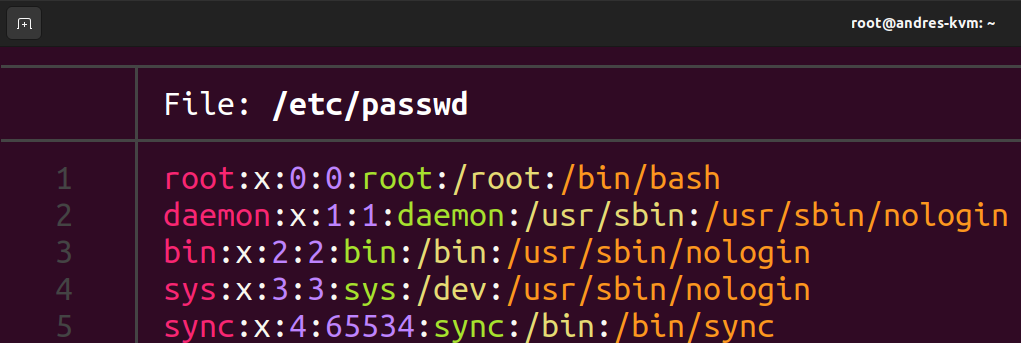
\includegraphics[width=\textwidth]{imagenes/passwdfile.png}
%    \caption{Ejemplo de entradas en el archivo.}
%\end{figure}

\end{document}
